\section{Setări}

Ecranul de setări controlează valorile predefinite utilizate în extragerea datelor despre bonuri și indicatorul care permite sau nu colectarea datelor. Modificarea acestor valori nu este inclusă explicit în domeniul aplicației, de aceea această funcționalitate este implementată numai la nivelul prezentării și infrastructurii. Interfețele definite de model, \texttt{CollectingOption} și \texttt{ReceiptDefaults} sunt implementate de clasa \texttt{PreferencesDao}, care este folosită pentru a accesa mediul de stocare \texttt{SharedPreferences}. 

\begin{figure}[h]
  \centering
  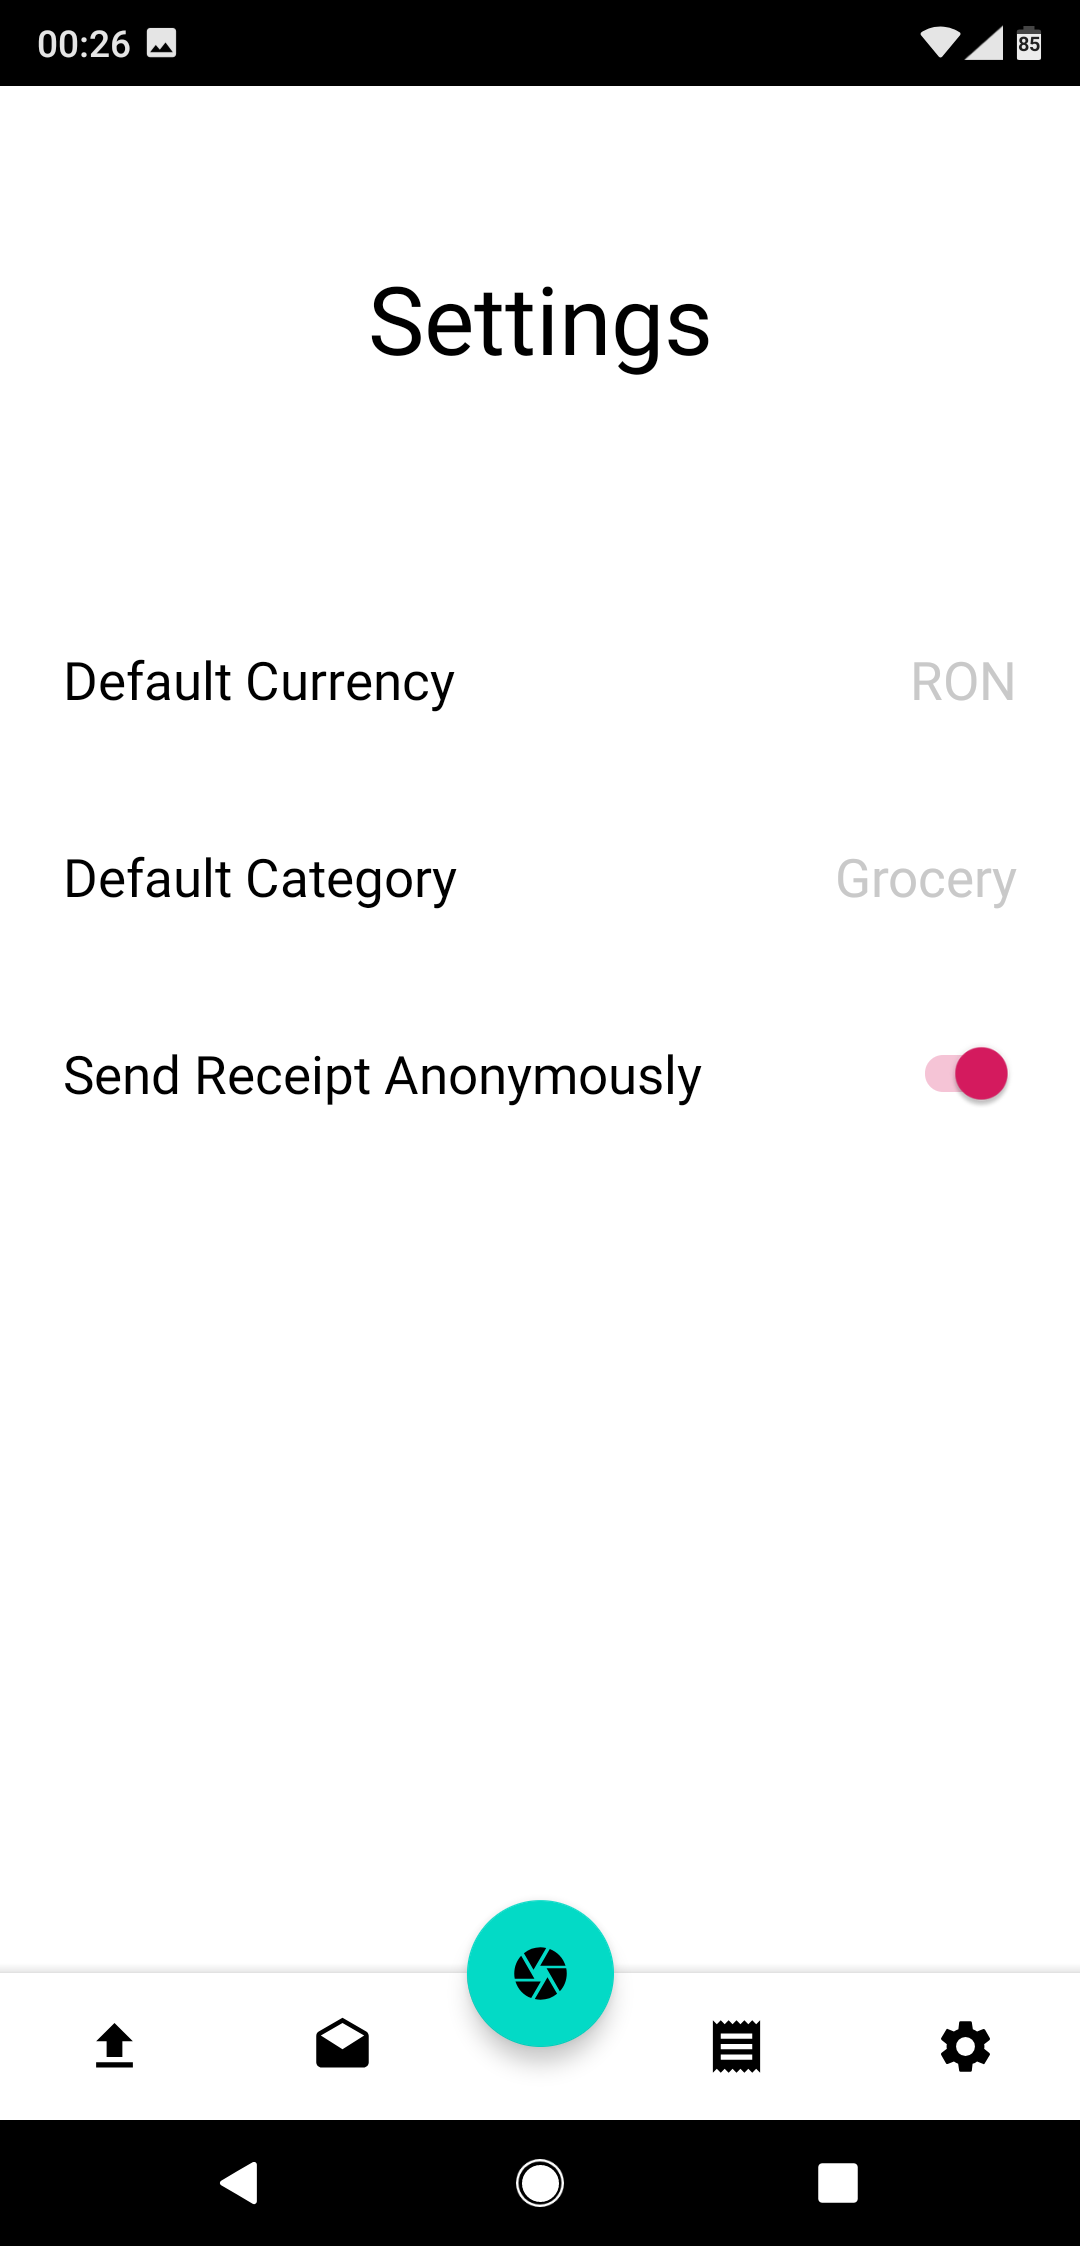
\includegraphics[width=\screenwidth]{SettingsScreen.png}
  \caption{Ecranul de setări}
  \label{settingsScreen}
\end{figure}